\documentclass[aspectratio=169,11pt]{beamer}

% Compile from the project root:
%   pdflatex presentation/course_presentation.tex
% Or compile from this presentation directory:
%   pdflatex course_presentation.tex

\usetheme{Madrid}
\usecolortheme{default}

\usepackage[T1]{fontenc}
\usepackage{lmodern}
\usepackage{amsmath}
\usepackage{amssymb}
\usepackage{booktabs}
\usepackage{graphicx}
\usepackage{array}

\graphicspath{{../figures/}{figures/}}

\definecolor{PaperBlue}{HTML}{1F4E79}
\definecolor{PaperTeal}{HTML}{2A7F73}
\definecolor{PaperGray}{HTML}{4A5568}
\definecolor{LightPanel}{HTML}{F4F7FA}

\setbeamertemplate{navigation symbols}{}
\setbeamertemplate{footline}[frame number]
\setbeamercolor{title}{fg=white,bg=PaperBlue}
\setbeamercolor{frametitle}{fg=white,bg=PaperBlue}
\setbeamercolor{structure}{fg=PaperBlue}
\setbeamercolor{block title}{fg=white,bg=PaperTeal}
\setbeamercolor{block body}{bg=LightPanel,fg=black}
\setbeamerfont{frametitle}{series=\bfseries}

\newcommand{\E}{\mathbb{E}}
\newcommand{\mui}[2]{\mu_{#1,#2}}
\newcommand{\Tij}[2]{T_{#1,#2}}

\begin{document}

\begin{frame}{Method: Why Matching Bandits?}
  \begin{columns}[T,onlytextwidth]
    \column{0.48\textwidth}
    \begin{block}{Classical bandit}
      \begin{itemize}
        \item A single learner chooses one arm each round.
        \item The chosen arm gives a stochastic reward.
        \item Exploration mainly affects this learner's own regret.
      \end{itemize}
    \end{block}

    \column{0.48\textwidth}
    \begin{block}{Matching bandit}
      \begin{itemize}
        \item Many agents compete for the same arms.
        \item Agents submit rankings, not direct choices.
        \item A platform converts rankings into a stable matching.
      \end{itemize}
    \end{block}
  \end{columns}

  \vspace{0.25cm}
  \begin{block}{Core innovation}
    \centering
    The paper studies bandit learning under stable matching constraints: learning errors can change market allocations.
  \end{block}
\end{frame}

\begin{frame}{Market Model and Stable Matching}
  \begin{columns}[T,onlytextwidth]
    \column{0.45\textwidth}
    \begin{block}{Market}
      \begin{itemize}
        \item Agent $i$ receives reward from arm $j$ with mean $\mu_{i,j}$.
        \item Agents learn means from repeated matches.
        \item Arms have fixed preferences over agents.
      \end{itemize}
    \end{block}

    \vspace{0.12cm}
    \begin{block}{Platform role}
      \centering
      rankings in, stable matching out
    \end{block}

    \column{0.50\textwidth}
    \begin{block}{Blocking pair}
      Pair $(i,j)$ blocks a matching if:
      \begin{itemize}
        \item $i$ prefers $j$ to its current arm;
        \item $j$ prefers $i$ to its current agent.
      \end{itemize}
    \end{block}

    \begin{block}{Stable matching}
      \centering
      stable matching = no blocking pair
    \end{block}
  \end{columns}

  \vspace{0.15cm}
  \begin{block}{Gale-Shapley platform}
    \centering
    submitted rankings
    \quad $\Longrightarrow$ \quad
    propose / hold / reject
    \quad $\Longrightarrow$ \quad
    stable matching $m_t$
    \quad $\Longrightarrow$ \quad
    observed rewards
  \end{block}
\end{frame}

\begin{frame}{UCB-GS Method}
  \begin{columns}[T,onlytextwidth]
    \column{0.48\textwidth}
    \begin{block}{Centralized setting}
      \begin{itemize}
        \item The platform observes all submitted rankings.
        \item It computes one global stable matching each round.
      \end{itemize}
    \end{block}

    \column{0.48\textwidth}
    \begin{block}{Per round}
      \begin{enumerate}
        \item Agents rank arms by UCB.
        \item Platform runs Gale-Shapley.
        \item Matched agents observe rewards.
        \item Observed pairs update estimates.
      \end{enumerate}
    \end{block}
  \end{columns}

  \vspace{0.15cm}
  \begin{block}{Ranking score}
    \[
      U_{i,j}(t)
      =
      \hat{\mu}_{i,j}(t)
      +
      \sqrt{\frac{3\log t}{2T_{i,j}(t-1)}}.
    \]
    \centering
    If $T_{i,j}(t-1)=0$, the arm is treated optimistically and explored first.
  \end{block}

  \vspace{0.1cm}
  \begin{block}{Two stable benchmarks}
    \centering
    agent-pessimal stable matching = worst stable outcome for agents\\[0.08cm]
    agent-optimal stable matching = best stable outcome for agents
  \end{block}
\end{frame}

\begin{frame}{Reproduced Experiments}
  \footnotesize
  \begin{tabular}{@{}p{0.16\textwidth}p{0.18\textwidth}p{0.18\textwidth}p{0.40\textwidth}@{}}
    \toprule
    \textbf{Figure} & \textbf{Market} & \textbf{Horizon / Trials} & \textbf{Purpose} \\
    \midrule
    1(a) & Example 2, $N=K=2$ & $n=400$, 100 trials per $\Delta$ & Test how a small gap for agent 1 affects agent 2 through matching. \\
    1(b) & Example 6, $N=K=3$ & $n=200$, 100 trials & Show that agent-optimal regret can be linear under UCB-GS. \\
    1(c) & Example 7, $N=K=20$ & $n=8000$, 50 trials & Compare regret patterns across high- and low-ranked agents. \\
    \bottomrule
  \end{tabular}

  \vspace{0.35cm}
  \begin{block}{Shared setup}
    Rewards are Gaussian with variance 1. The plots use expected cumulative regret computed from the true mean rewards.
  \end{block}
\end{frame}

\begin{frame}{Figure 1(a): Small Gap, Large Spillover}
  \begin{columns}[T,onlytextwidth]
    \column{0.60\textwidth}
    \centering
    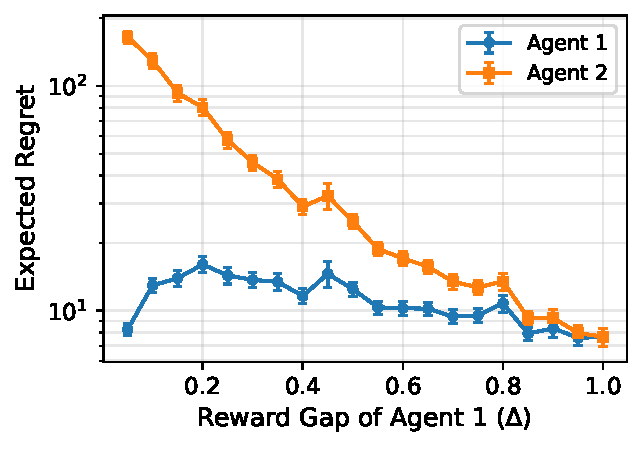
\includegraphics[width=\linewidth,height=0.70\textheight,keepaspectratio]{figure_1a.pdf}

    \column{0.36\textwidth}
    \begin{block}{Takeaway}
      \centering
      When agent 1's reward gap is small, its slow learning can create large regret for agent 2.
    \end{block}
  \end{columns}
\end{frame}

\begin{frame}{Figure 1(b): Linear Regret}
  \begin{columns}[T,onlytextwidth]
    \column{0.60\textwidth}
    \centering
    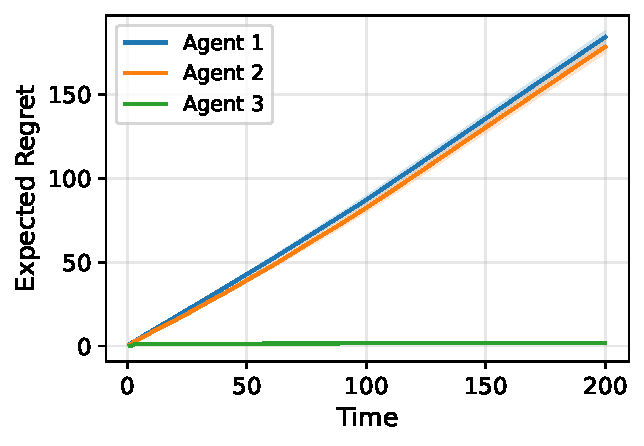
\includegraphics[width=\linewidth,height=0.70\textheight,keepaspectratio]{figure_1b.pdf}

    \column{0.36\textwidth}
    \begin{block}{Takeaway}
      \centering
      Agent-optimal regret can be nearly linear, even though UCB-GS is designed for the agent-pessimal benchmark.
    \end{block}
  \end{columns}
\end{frame}

\begin{frame}{Figure 1(c): Global Preferences}
  \begin{columns}[T,onlytextwidth]
    \column{0.60\textwidth}
    \centering
    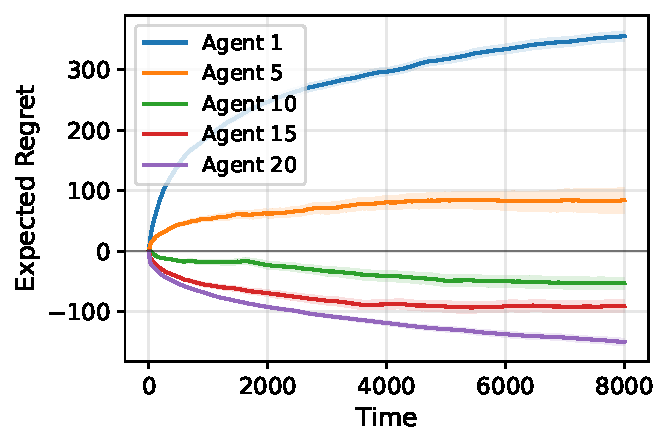
\includegraphics[width=\linewidth,height=0.70\textheight,keepaspectratio]{figure_1c.pdf}

    \column{0.36\textwidth}
    \begin{block}{Takeaway}
      \centering
      Lower-ranked agents can have negative regret because exploration may temporarily give them better arms.
    \end{block}
  \end{columns}
\end{frame}

\end{document}
